
% Appendix Template
\chapter{eSNN Architectures for Stock Price Movement Forecast}
\label{app:eSNN_stock}

In the last few years, there have been a large number of studies performed on predicting the stock market trend. Both researchers and practitioners have used numerous approaches to predict the stock market trend. Due to the chaotic nature and the complexity of the stock market indices, researchers are still struggling to design techniques that can accurately model the behaviour of their trends. In \tablename \ref{tab:techniques_in_litrature}, we have given an overview of the different prediction techniques and stock market indices used in the literature to predict the stock price direction by taking technical indicators as input variables. 

\tablename \ref{tab:techniques_in_litrature} presents a concise literature review on machine learning techniques applied on stock price movement prediction. It is clear that many traditional machine learning techniques have been explored to predict stock price direction and also most of the algorithms have been applied to a single stock index to measure the performance of the model. In the third generation of neural networks the spiking neural networks (SNN) now offers a new perspective to explore for the solution of the problem. SNN uses spike information representation and spike-time learning rules to capture temporal associations between a large number of temporal variables in streaming data and to predict future events. One of the successful SNN models is the eSNN model, where the number of spiking neurons evolve incrementally in time to capture temporal prototypes from data.  

\section{The SI-eSNN Model for Stock Trend Prediction Based on Stock Indicators}
\begin{figure}
	\centering
	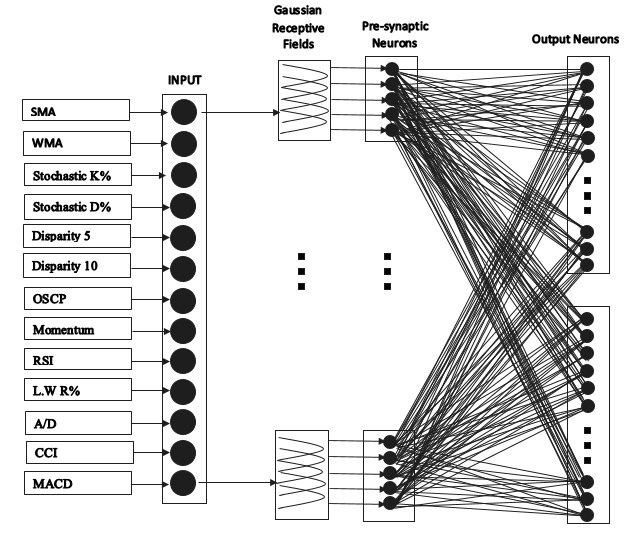
\includegraphics[scale=0.5]{fig/snn/esnn_arch.PNG}
	\caption{Architecture of the proposed technical stock indicator SI-eSNN model for stock price direction prediction}
	\label{fig:esnn_arch_stock}
\end{figure}

\subsection{Overall Architecture}

The architecture of the SI-eSNN model is presented in \figurename \ref{fig:esnn_arch_stock}. The first layer is the set of inputs to the model, each of them representing a technical stock indicator. The research so far has demonstrated that using technical indicators can lead to better results than using real stock values as time series and also that there is a lot of research done on selecting the most appropriate technical indicators. In the model presented in
\figurename \ref{fig:esnn_arch_stock} the input technical indicators have been selected from \citep{patel2015predicting, kim2003financial, kara2011predicting} and explained in \tablename \ref{tab:tech_indicators}, but these indicators can vary across stock prediction applications.


\footnotetext{$C_t$ is the closing price, $L_t$ is the low price and $H_t$ is the high price at time $t$, $DIFF_t=EMA(12)_t-EMA(26)_t$, $EMA$ is the moving average, $EMA(k)_t=EMA(k)_{t-1}+\alpha \times (C_t- EMA(k)_{t-1})$, $\alpha$ is the smoothing factor which is equal to $\frac{2}{k+1}$, $k$ is the time period of k-day exponential moving average, $LL_t$ and $HH_t$ implies lowest low and highest high in the last $t$ days respectively. $M_t=\frac{H_t+L_t+C_t}{3}$, $SM_t=\frac{\sum_{i=1}^n M_{t-i+1}}{n}$, $D_t=\frac{\sum_{i=1}^n |M_{t-i+1}-SM_t|}{n}$, $UP_t$ means upward price change while $DW_t$ is the downward price change at time $t$}.

Layer 2 is the encoding layer, where the real value of each input variable (technical indicator) is encoded as trains of spikes generated by several encoding spiking neurons (or also, pre-synaptic neurons), each of them having a receptive field. The receptive fields of neighbouring neurons are overlapping as Gaussian or Logistic functions and all of them covering the whole range of the values of this variable. The number of these encoding neurons (receptive fields) can vary, and this is a user-defined parameter that is optimised for a better performance
of the model.

Layer 3 is the output evolving layer, which evolves output spiking neurons that represent clusters (prototypes) of input vectors that belong to the same class, in this case class UP and
class DOWN. Each output neuron is connected to all the input neurons, and the connection weights are subject to learning from data.

The architecture of the SI-eSNN model for stock price direction prediction allows for incremental learning. It is adaptive to new data when it becomes available. Hence, it can learn new samples without retraining the model on old data. The details of the functioning of the SI-eSNN model is
presented below.

\subsection{Neural Encoding}

To learn real-valued data, each instance or sample (input vector) is encoded in the form of spikes over time using a neural encoding technique such as rank order population coding \citep{thorpe1997rapid,bohte2002error}. In our study, we have used rank order population encoding as per \citep{schliebs2009integrated}. Population encoding maps the input value into a series of spikes over time using an array of Gaussian receptive fields that describe pre-synaptic neurons. The center ($C_j$) and width ($W_j$) of each of the Gaussian or Logistic receptive field of pre-synaptic neurons $j$ are defined as:

\begin{equation}
C_j=I_{min}^n + \frac{2j-3}{2}\times \frac{I^n_{max}-I^n_{min}}{N-2}
\end{equation}

and 

\begin{equation}
W_j=\frac{1}{\beta}\times \frac{I^n_{max}-I^n_{min}}{N-2}, 1\leq \beta \leq 2
\end{equation}

Where N is the number of receptive fields; n is the range of input variable $n = [I_{min}^n, I_{max}^n ]$ , the parameter $\beta$ defines the width of each receptive field. Output of each of the pre-synaptic neuron $j$ using Gaussian receptive field is defined as:

\begin{equation}
output_j=\exp(-\frac{(x-C_j)^2}{2\cdot W_j^2})
\end{equation}

Output of each of the pre-synaptic neuron $j$ using Logistic receptive field is defined as:

\begin{equation}
output_j=\frac{\exp(\frac{-(x-C_j)}{W_j})}{(1+\exp(\frac{-(x-C_j)}{W_j}))^2}
\end{equation}

The firing time of each of the pre-synaptic neurons is defined as:

\begin{equation}
\tau_j=\floor{T(1-output_j)}
\end{equation}

where: $T$ is the simulation or spike time interval.

When a real value input is presented to the N pre-synaptic spiking neurons, the first spike is generated by this neuron to which receptive field the input value belongs to the highest  degree, etc.  



\subsection{Neural Model}

For the context of SI-eSNN, Thorpe’s neuron model \citep{thorpe1997rapid} has been used since it is simple and effective. The Thorpe’s model is based on the timing of each spike, that is, earlier spike defines stronger weight as compared to the later spike. Each neuron in this model can spike at most once. A neuron in this model fires when it’s post-synaptic potential (PSP) reaches the threshold value. The PSP of neuron $i$ is defined as:

\begin{equation}
PSP_i=
\begin{cases}
0, & \text{if}\ fired \\
\sum w_{ji}*mod^{order(j)}, & \text{otherwise}
\end{cases}
\end{equation}

Where  $w_{ji}$ represents the weight of the synaptic connection between pre-synaptic neuron $j$ to the output neuron $i$; $mod$ represents modulation factor with a range in between 0 to 1; $order(j)$ defines the rank of pre-synaptic neurons spike. The first rank will be assigned as 0 and subsequently, rank will be increased by 1 based on firing time of each pre-synaptic neurons. 

\subsection{Learning in the Output Neurons}

The eSNN algorithm was first introduced in \citep{wysoski2006adaptive,kasabov2007evolving}. The learning techniques used by the eSNN model is one-pass learning, that is, the model requires one-time presentation of a sample in a feed-forward manner. It will create an output neuron for each input sample. The weight vector and a threshold value for each of the output neuron generated towards the training pattern are learned and stored in the repository. However, if this weight vector is similar to the weight vector of the already trained neuron in the repository with some similarity threshold, then it will merge with the most similar one. Merging here means updating the weights and the threshold value of the merged neurons. The weight vector and threshold value of the merged neurons update their values by taking the average value of new output neuron weight vector and merged neuron weight vector and the average value of new output neuron threshold and merged neuron threshold respectively. 

\subsection{Algorithm for eSNN Training}

\begin{algorithm}
	\begin{algorithmic}[1]
		\STATE Initialize neuron repository, $R=\{\}$
		\STATE Set eSNN parameter $mod=[0, 1], C= [0, 1], sim=[0, 1]$
		\FOR{$\forall$ input pattern $i$ that belongs to the same class}
		\STATE Encode input pattern into firing time of multiple pre-synaptic neurons $j$
		\STATE Create a new output neuron $i$ for this class and calculate the connection weights as $w_{ji}=mod^{order(j)}$
		\STATE Calculate $PSP_{max(i)}=\sum_j w_{ji}\times mod^{order(j)}$
		\STATE Get $PSP$ threshold value $\gamma_i = PSP_{max(i)}\times C$
		\IF{The new neuron weight vector $\leq$ $sim$ of trained output neuron weight vector in $R$}
		\STATE Update the weight vector and threshold of the most similar neuron in the same output class group
		\STATE $w=\frac{w_{new}+w*N}{N+1}$
		\STATE $\gamma=\frac{\gamma_{new}+\gamma*N}{N+1}$
		\STATE where $N$ is the number of previous merges of the most similar neuron
		\ELSE
		\STATE Add the weight vector and threshold of the new neuron to the neuron repository $R$
		\ENDIF
		\ENDFOR
		\STATE Repeat above for all input patterns of other output classes
	\end{algorithmic}
	\caption{eSNN training algorithm}
	\label{alg:esnn}
\end{algorithm}

The eSNN algorithm creates a repository of output neurons for the training patterns. For each training pattern that belongs to the same class, a new output neuron is created and connected to all the pre-synaptic neurons in the previous layer. The weight for each of the connection from pre-synaptic neuron $j$ to output neuron $i$ is denoted as $w_{ji}$. The value of $w_{ji}$ is calculated based on the spike order through a synapse $j$, which is given in line 5 of \algorithmname \ref{alg:esnn} as $w_{ji}=mod^{order(j)}, \forall j$ where $j$ is the pre-synaptic neuron of output neuron $i$.

The threshold $\gamma_i$  of newly created output neuron would be defined as the fraction $C \in \mathbb{R},0<C<1$, of the maximum post-synaptic potential $PSP_{max⁡(i)}$: $\gamma_i = PSP_{max(i)}\times C$

The weight vector of newly created output neuron is then compared with the already trained output neurons in the repository. If the newly created output neuron weight vector is less than $sim$ of trained neuron weight vectors, then the threshold and weight vector of newly created output neuron is merged with most similar neuron according to $\displaystyle w=\frac{w_{new}+w*N}{N+1}$ and $\displaystyle \gamma=\frac{\gamma_{new}+\gamma*N}{N+1}$.

Here, $N$ is the number of previous merges of the most similar neurons. After the merge operation, the newly created output neuron weight vector is discarded, and the new pattern is presented to model. If none of the trained neurons in the repository is similar, the new output neuron is added to the repository.


\subsection{Testing (Recall of the Model on New Data)}

The testing process is done by propagating the spikes that encode the test vector (sample) to all trained output neurons. The class label for the testing sample will be defined based on the output class label of the output neuron which fires first.


\section{The CUDA-SI-eSNN Model: A Parallel eSNN Model for GPU Machines}
\label{sec:cuda_esnn}

\begin{algorithm}
	\begin{algorithmic}[1]
		
		\STATE Initialize input patterns array in device memory with size is equal to $N \times M$, Where $N$ is number of input patterns and $M$ is number of input variable.
		
		\STATE Declare weights matrix in device memory with size is equal to $N \times P$
		Where $P$ is number of pre-synaptic neurons which is equal to the number of input variable multiplied by number of Gaussian receptive fields.
		
		\STATE Transfer the input patterns data into the GPU memory.
		
		\STATE Encode input patterns into firing time of multiple pre-synaptic neurons $j$. In this step, each of the threads in the GPU device will calculate the firing-time of each of the pre-synaptic neurons independently. The number of threads is equal to $N \times P$.
		
		\STATE Calculate the connection weights as  $w_{ji}=mod^{order(j)}$. In this step, each tread in the GPU device will calculate the weight independently.
		
		\STATE Transfer the resulted weight matrix into CPU memory.
		
		\STATE Calculation of maximum post-synaptic potential $PSP_{max⁡(i)}$, 	threshold value $\gamma_i$ and the 	merging operation are similar to the equivalent operations of eSNN, which are performed on CPU sequentially.
	\end{algorithmic}
	\caption{CUDA-SI-eSNN algorithm}
	\label{alg:cuda_esnn}
\end{algorithm}

The training and recall procedures for the SI-eSNN model consists of two operations. In the first stage, encoding of the input patterns, calculations of the weights and the thresholds are performed, which is from step-4 to step-7 of the eSNN algorithm. In the second stage, merging of the output neurons is performed, which is from step-8 to step-14 of the eSNN algorithm. Since the encoding and learning of weights of one input pattern is independent of others except for the merging operation, it is possible to perform both encoding and weight learning operations parallelly in GPU device using multiple threads. The procedure for the GPU-based eSNN algorithm is described in \algorithmname \ref{alg:cuda_esnn}.

\section{Sliding Window (SW)-eSNN for Incremental Learning and Stock Movement Prediction}
\label{sec:sw_esnn}
\begin{algorithm}
	\begin{algorithmic}[1]
		
		\STATE Train an eSNN model on the whole existing historical data of a stock till time $t$ (as per \algorithmname \ref{alg:esnn})
		\STATE Recall the model to predict the next month (t+1) stock movement.
		\STATE When the next month results are known, train the model incrementally on this data.
		\STATE Aggregate the output neurons if necessary using the aggregation operator and the $sim$ parameter. 
		\STATE Evaluate the classification error and the AUC so far. 
		\STATE Optimize parameters to improve future time accuracy.
	\end{algorithmic}
	\caption{SW-eSNN learning algorithm}
	\label{alg:sw_esnn}
\end{algorithm}

While learning in the SI-eSNN and CUDA-SI-eSNN models were vector by vector and each vector was learned separately from the others even though the vectors of consecutive days would have some temporal associations. Here we present an SW-eSNN model where a window based block of the time series of technical indicator data is used for training a model and a future section – to test it. Then the window moves in time, to select the next section for training and testing, etc. 


\begin{sidewaystable}
	\centering
	\caption{Prediction Techniques and Stock Market Indices for Stock Price Direction Prediction used in Literature}
	\label{tab:techniques_in_litrature}
	\resizebox{\textwidth}{!}{\begin{tabular}{llll}
			\toprule[1.25pt]
			& Techniques                                          & Stock Market Indices                                              & GPU-Based \\
			\midrule
			\citep{chiou1996applying}   & RNN                                                 & TSI                                                               & No        \\
			\citep{tsaih1998forecasting}   & RBS + RNN                                           & S \& P 500                                                        & No        \\
			\citep{saad1998comparative}   & TDN, RN, PNN                                        & AAPL, IBM, MOT, MSFT                                              & No        \\
			\citep{kim2000genetic}    & GA + ANN                                            & KOSPI                                                             & No        \\
			\citep{kim2003financial}    & SVM                                                 & KOSPI                                                             & No        \\
			\citep{kim2004stock}   & FS + ANN                                            & KOSPI                                                             & No        \\
			\citep{huang2005forecasting}    & SVM, LDA, QDA, EBNN                                 & Nikkie-225                                                        & No        \\
			\citep{kumar2006forecasting}   & RF , SVM                                            & NIFTY, CNX, S \& P 500                                            & No        \\
			\citep{huang2008application}   & Wrapper, LR, SVM, C 4.5 DT, BP, KNN, Voting         & KOSPI, TSE                                                        & No        \\
			\citep{ou2009prediction}   & LDA, QDA, KNN, NB, SVM, LS-SVM, ANN, TBC, BC, Logit & HSI                                                               & No        \\
			\citep{zhang2009stock}   & IBCO + BPNN                                         & S \& P 500                                                        & No        \\
			\citep{mostafa2010forecasting}   & MLP, GRNN                                           & KSE                                                               & No        \\
			\citep{nair2010decision}   & DT + RS                                             & BSE                                                               & No        \\
			\citep{kara2011predicting}   & SVM, ANN                                            & ISE                                                               & No        \\
			\citep{chang2012novel}   & EPCNNs                                              & S \& P 500                                                        & No        \\
			\citep{lin2013svm}   & SVM                                                 & TW50                                                              & No        \\
			\citep{de2013applying}   & ANN                                                 & PETR4                                                             & No        \\
			\citep{wang2014stock}   & PCA  + SVM                                          & KOSPI, HSI                                                        & No        \\
			\citep{bisoi2014hybrid}   & ANN                                                 & BSE, IBM, RIL, OSI                                                & No        \\
			\citep{patel2015predicting}    & ANN, SVM, NB, RF                                    & NIFTY, BSE-Sensex, Infosys, Reliance                              & No        \\
			\citep{hafezi2015bat}   & BNNMAS                                              & DAX                                                               & No        \\
			\citep{ballings2015evaluating}    & LR, ANN, KNN, SVM, AB, RF, KF                       & European Stock Index                                              & No        \\
			\citep{zhang2016stock}    & AB + PSVM +GA                                       & SZSE, NASDAQ                                                      & No        \\
			Our study & eSNN, CUDA-eSNN                                     & BSE, NIFTY-50, NASDAQ, Nikkie-225, DAX, NYSE-Amex,S \& P-500, SSE & Yes \\
			\bottomrule[1.25pt]     
	\end{tabular}}
\end{sidewaystable}

\begin{table}
	\centering
	\caption{Selected technical indicators and their formulas}
	\label{tab:tech_indicators}
	\resizebox{\textwidth}{!}{%
		\begin{tabular}{|l|l|}
			\toprule[1.25pt]
			Name of the technical indicators (SI)        & Formulas \footnotemark \\
			\midrule
			Simple 10-day moving average                 &   $\displaystyle \frac{C_t+C_{t-1}+\cdots +C_{t-9}}{10}$       \\
			Weighted 10-day moving average               &   $\displaystyle \frac{(n)\times C_t+(n-1)\times C_{t-1}+\cdots+C_{t-9}}{(n+(n-1)+\cdots+1)}$       \\
			Stochastic K\%                               &    $\displaystyle \frac{C_t-LL_{t-(n-1)}}{HH_{t-(n-1)}-LL_{t-(n-1)}}\times 100$      \\
			Stochastic D\%                               &  $\displaystyle \frac{\sum_{t=0}^{n-1}K_{t-i}}{10}\%$        \\
			Disparity 5                                  &    $\displaystyle \frac{C_t}{MA_5}\times 100$      \\
			Disparity 10                                 &    $\displaystyle \frac{C_t}{MA_{10}}\times 100$       \\
			OSCP                                         &     $\displaystyle \frac{MA_5-MA_{10}}{MA_{10}}$     \\
			Momentum                                     &     $\displaystyle C_t-C_{t-9}$    \\
			RSI (Relative Strength Index)                &     $\displaystyle 100-\frac{100}{1+\frac{\sum_{i=0}^{n-1}UP_{t-i}/n}{\sum_{i=0}^{n-1}DW_{t-i}/n}}$  \\
			
			
			Larry William R\%                            &      $\displaystyle \frac{H_n-C_t}{H_n-L_n}\times 100$    \\
			A/D (Accumulation/Distribution)              &      $\frac{H_t-C_{t-1}}{H_t-L_t}$    \\
			CCI (Commodity Channel Index)                &       $\frac{M_t-SM_t}{0.015\times D_t}$   \\
			MACD (moving average convergence divergence) &       $MACD(n)_{t-1}+\frac{2}{n+1}\times (DIFF_t- MACD(n)_{t-1})$   \\
			\bottomrule[1.25pt]
			
	\end{tabular}}
\end{table}

\begin{table}
	\centering
	\caption{The number of instances of UP and DOWN categories in Stock Market Indices}
	\label{tab:num_instance_up_down}
	\resizebox{\textwidth}{!}{\begin{tabular}{@{}cccccccc@{}}
			\toprule
			Datasets (No. of instances) & Years Covered         & \multicolumn{3}{c}{Training (70\%)} & \multicolumn{3}{c}{Testing (30\%)} \\ \midrule
			&                       & UP         & Down      & Total      & UP        & DOWN      & Total      \\ \midrule
			BSE                         & Jan 2005- Dec 2015    & 1020       & 892       & 1912       & 437       & 382       & 819        \\
			Nikkie-225                  & Jan 1987 - Jul 2016   & 2609       & 2483      & 5092       & 1115      & 1067      & 2182       \\
			NASDAQ                      & Jan 2005 - Dec 2015   & 1058       & 865       & 1923       & 446       & 378       & 824        \\
			NIFTY-50                    & Jan 2008 - Dec 2015   & 709        & 644       & 1353       & 300       & 279       & 579        \\
			S\&P-500                    & Jan 1962 - July 2016  & 5118       & 4473      & 9591       & 2146      & 1964      & 4110       \\
			Sanghai Stock Exchange      & Jan 1998 - July 2016  & 1679       & 1470      & 3149       & 685       & 665       & 1350       \\
			DJUS                        & Apr 2005 - July 2016  & 997        & 827       & 1824       & 438       & 344       & 782        \\
			DAX Index                   & Jan 1991 - July 2016  & 2413       & 2114      & 4527       & 1044      & 897       & 1941       \\
			NYSE-Amex                   & Jan 1996 to July 2016 & 1957       & 1668      & 3625       & 850       & 704       & 1554       \\ \bottomrule
	\end{tabular}}
\end{table}

\begin{table}
	\centering
	\caption{GPU Specifications}
	\label{tab:gpu_specs}
	\begin{tabular}{ll}
		\toprule[1.25pt]
		\multicolumn{2}{c}{GeForce GT 730 Specifications}  \\
		\midrule
		Version                    & GT 730  DDR3, 64-bit  \\
		CUDA Cores                 & $384$                   \\
		Base Clock (MHz)           & $902$                   \\
		Memory Clock               & $1.8$ Gbps              \\
		Standard Memory Config     & $2048$ MB               \\
		Memory Interface           & DDR3                  \\
		Memory Interface Width     & 64-bit                \\
		Memory Bandwidth (GB/sec)  & $14.4$                  \\
		\bottomrule[1.25pt] 
	\end{tabular}
\end{table}




